\documentclass{scrartcl}

\usepackage{graphicx}

\title{Sensing Senses}
\subtitle{Correlations Between Image Features and Neural Spikes}
\author{C.M. Lubinski}

\begin{document}
\maketitle

\begin{abstract}
What types of images excite the brain? By correlating features of images with
neural spikes, we can begin to answer this question. Several potential
features for images, along with a method of determining statistically
significant correlations are provided. They are used against an existing
experimental data set, determining the most relevant features for that study.
Potential flaws and tests for accuracy of these correlations are also
discussed.
\end{abstract}

\section{Experimental Data}
The data set we will use to test our method comes from David Sheinberg's lab
at Brown University. During the deriving experiment, a sensor was placed in a
test subject's inferior temporal cortex. Images of various, individual objects
were displayed on a screen within the subject's sight while its neural
activity was recorded. As this area of the brain is known to be associated
with object recognition, we expect different objects to elicit different spike
rates. 

The experiment was ran over three days, with two test subjects. We do not know
if the sensor's location moved between days, nor do we know the subject's
familiarity with the displayed objects. We chose to proceed with only one
day's results, as spanning days and/or subjects may not provide comparable
data. The second day's dataset was chosen as it has the most data points.

\section{Finding Features}

Effectively, we begin this study with a collection of neural spikes and the
images that were on screen when those spikes occurred. To determine which
features of these images are most relevant to the spike rate, we will need to
decompose the images into their component features. This task is challenging,
however, as images can be described (i.e. converted into features) in a
limitless number of ways -- a picture is worth a thousand words, alone. Our
chosen set of potential features will therefore directly limit which
correlations we can derive.

Recognizing that we cannot be complete, we will start with the simplest
features and slowly expand in to the sophisticated. The most obvious
attributes of an image, at least a digitized image, are the red, green, blue,
and transparent (``alpha'') values for each pixel. To convert these individual
values into something which applies to the entire image, we will calculate the
{\em average} red, green, blue, and alpha values for the image as a whole.
Though simple, one of these will prove to be one of the most statistically
significant correlations.

The colors we perceive are combinations of these values, however. The color
``yellow'' may lead to more neural activity than red, green, or blue alone. We
should therefore combine our primary colors through addition, multiplication,
and divisions of their average hues. Here, great caution is warranted; testing
tens of thousands of permutations raises the risk of misleading statistical
significance. A correlation with $p$ value of $0.01$ will, {\em by
definition}, erroneously appear roughly ten times if we test a thousand
features. To minimize this risk, we limit the number of color combinations we
will test.

The feature set defined by each image's average colors will be very useful,
but it is a bit blunt. As the neurons studied are associated with {\em
recognition}, we will also look for more abstract features. We convert each
image into grey-scale and then look for how much of the screen is actually
comprised of "image" and how much is blank, by checking for the ``presence''
of individual pixels (evident by having a non-background color). We also
compare each pixel to its neighbors to determine an average
``difference''/``sameness'' for the entire image. We also include counting the
number of times three pixels are ``present'' in a row or column to determine a
metric of verticality/horizontal-ness for the image as a whole. Each metric is
devised as a simple loop which adds values for each pixel in the image. This
sum is then divided by the area of the entire image to determine an average.

We went further, making very blunt use of cutting-edge computer vision
techniques provided by the {\ttfamily skimage} package from scikit. Assuming
we used this library correctly, we included the number of ``corners'' present
in an image (using the Harris algorithm), and the number of ``blobs'' (via the
Difference of Gaussian approach). We use these features as tech demos more
than anything else, though skimming the research behind them has been quite
fascinating.

In summary, in addition to combinations of colors, we have the following base
features:

\begin{center}
\begin{tabular}{| l | l |}
  \hline
  Feature & Description\\
  \hline
  red & Average hue of red\\
  green & Average hue of green\\
  blue & Average hue of blue\\
  alpha & Average intensity of alpha\\
  present & Average non-background pixels\\
  horiz & Average ``horizontal'' rating\\
  vert & Average ``vertical'' rating\\
  diff & Average difference between adjacent pixels\\
  blob & Number of blobs (Difference of Gaussian)\\
  corners & Number of corners (Harris)\\
  \hline
\end{tabular}
\end{center}

\section{Deducing Correlations}

Once we have a set of features, we can test each feature against the spike
rates encountered. We will look for {\em correlations} between each feature
and spike rate by calculating a correlation coefficient, using the
{\ttfamily scipy.stats.spearman} function. Correlations which are
statistically significant (as determined by having a $p$ value less than
$0.05$ over the number of features tested) are kept, while the majority are
cut. The remaining features are then sorted to see which have the largest
effect on the spike rate.

To calculate correlation coefficient, we will need to quantify how individual
images include such features. For some features, we need only boolean `0' and
`1' values, as we only care about the feature's presence. For others, we will
need a scale, preferably normalized to the zero-to-one range. We will use the
Spearman correlation algorithm, which does not require the data be linear and
is more forgiving about normalization than many other algorithms (e.g.
Pearson's algorithm).

Here, we should take a brief moment to describe a problem that plagued this
work for quite some time. With just enough knowledge to be dangerous, our
initial effort attempted to use machine learning techniques to determine which
features were most relevant. This lead us down winding roads hinting at
regression models, linearity, feature decomposition, and a wealth of other
minutia which repeatedly gave us no usable results. These systems can no doubt
be used to solve our problem, but we lacked the knowledge to use them
effectively. Always start with a simple strategy rather than wasting time on
more delicate, advanced techniques.

\section{Results}

For the data set in question, we found some surprising results. The majority
of our features have no statistically significant correlation with spike rate.
The somewhat abstract features, such as blob detection, internal similarity,
and verticality, are no where to be seen.  The features which {\em are}
present correlate relatively well, with between 20 and 30\% correlation
coefficients. 

\begin{figure}[h]
  \centering
  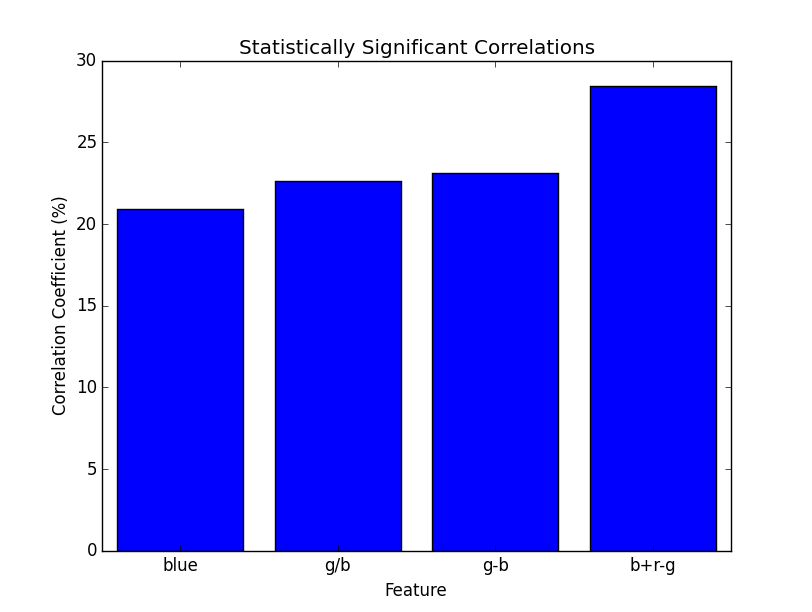
\includegraphics[width=3in]{significance.png}
\end{figure}

While the color blue clearly correlates with heightened neural activity, the
combinations give a slightly more detailed perspective. When the ratio between
green and blue is high (creating either a green or yellow hue), neurons appear
to fire less often. When the blue and red are present but green is absent
(creating purple), the neurons are most excited. 

\begin{figure}[h]
  \centering
  
\includegraphics[width=3in]{spectrum.png}
  \caption{Least to Most Stimulating Colors (In This Study)}
\end{figure}

\section{Verifying the Method}

How do we know that these features are the strongest influencers of neural
activity? Clearly we cannot compare these features to those which we did not
consider, but can we know whether our method ``worked'' {\em within} the
features we chose?

Our first instinct would be to run the same test using one of the other data
sets. The third dataset is too small, but we can try our method on the first.
Unfortunately, the results are drastically different, with only the ratio
between red and green statistically significant. So what went wrong? On the
forgiving hand, the two data sets come from two different sensors in two
different subjects; they simply are not comparable. On the more probable hand,
the authors must recognize that our knowledge of statistical methods is
limited; we no doubt made several mistakes.

At the very least, we can throw some ``sanity'' tests at our algorithm; these
are junk features which have an expected outcome. Our feature decomposition
will include these features and should give an expected correlation for each.
``Constant'' features, which always return zero or always return one, should
have very low correlation. A feature composed of random values may have some
correlation, but should not be statistically significant. Correlating the
spike count with itself should provide a perfect correlation coefficient.
Luckily, when we test our method with these features, we see that it passes
each with expected values.

\section{Next Steps}

The method described hinges on the types of features we can devise from each
image. To find stronger correlations, we need to develop more sophisticated
features. In particular, we know that the portion of the brain measured is
related to image {\em recognition}, so knowledge of the subject's familiarity
with each image would be immensely valuable. Labeling images with other
suspected patterns, such as the presence of ``eyes'' in the image or the
perspective with which the image was taken could also correlate to neural
activity.

As with any statistical analysis, the more data with which we have access, the
more accurate our results will be. To develop the most robust model, we would
want to track the neural pulses through millions of images. While the
described experiment could be extended by a small factor, displaying single
images on the screen cannot scale. A more alluring alternative would be to
place a camera on the subject's head to capture their line of sight. If a
long-term neural sensor could be installed, we could look for features and
spikes within small time spans. This would be messy, but would scale in ways
the single-image approach could not.

\section{Thank You}

This exploration took place as part of Monica Linden and David Sheinberg (both
of Rice University)'s Coursera course, "Exploring Neural Data". It makes
direct use of Sheinberg's data and snippets of code provided by both. The
course is excellent; I recommend it to anyone with some programming skill who
is interested in the brain.

All source code for this project is available on GitHub:

{\ttfamily https://github.com/cmc333333/neuraldata-final}

\end{document}
